\section{Results}
\label{sec:results}

This section presents the experimental results according to the research questions introduced in Section~\ref{sec:introduction}. The main research question is addressed through three sub research questions. Each subsection presents the experimental evidence corresponding to one sub research question. The implications of these findings are discussed in Chapter~\ref{sec:discussion}.


\subsection{Main Research question}
\label{subsec:mainrq}
The following subsections present the experimental evidence used to answer the main research question regarding the comparison between YOLOv8 and LLaVA 1.6 for housing inspection.

\subsubsection{SRQ1 Comparison of YOLOv8 and LLaVA 1.6}
\textbf{SRQ1:} How do YOLOv8 and LLaVA 1.6 compare in detecting and identifying inspection relevant categories using shared evaluation?


To establish a reference point, baseline configurations of both models were evaluated. Property 001 was selected as an initial benchmark because it contains only inspection relevant issues and therefore provides a clear indication of whether the models can correctly identify housing defects.

Table~\ref{tab:gt_property001} shows the ground truth distribution of Property 001. The dataset consists of six damage images and four wear images, while no images belong to the no damage category.

% 
% Table truth labels property 1 
\begin{table}[H] \centering \caption{Ground truth distribution for property 001} \label{tab:gt_property001} \begin{tabular}{lc} \toprule Category & Number of images \\ \midrule Damage & 6 \\ Wear & 4 \\ No damage & 0 \\ \midrule Total & 10 \\ \bottomrule \end{tabular} \end{table} 
%                                         

Figure~\ref{fig:baseline_heatmaps} presents the confusion matrices of the baseline models. The LLaVA baseline predominantly classified images as no damage, resulting in poor recognition of inspection relevant categories. The YOLOv8 baseline achieved stronger category separation, although substantial misclassifications remained. These baseline results indicate that additional optimization is required for both approaches.

%                          

\begin{figure}[H]
\centering

\begin{subfigure}{0.9\columnwidth}
\centering
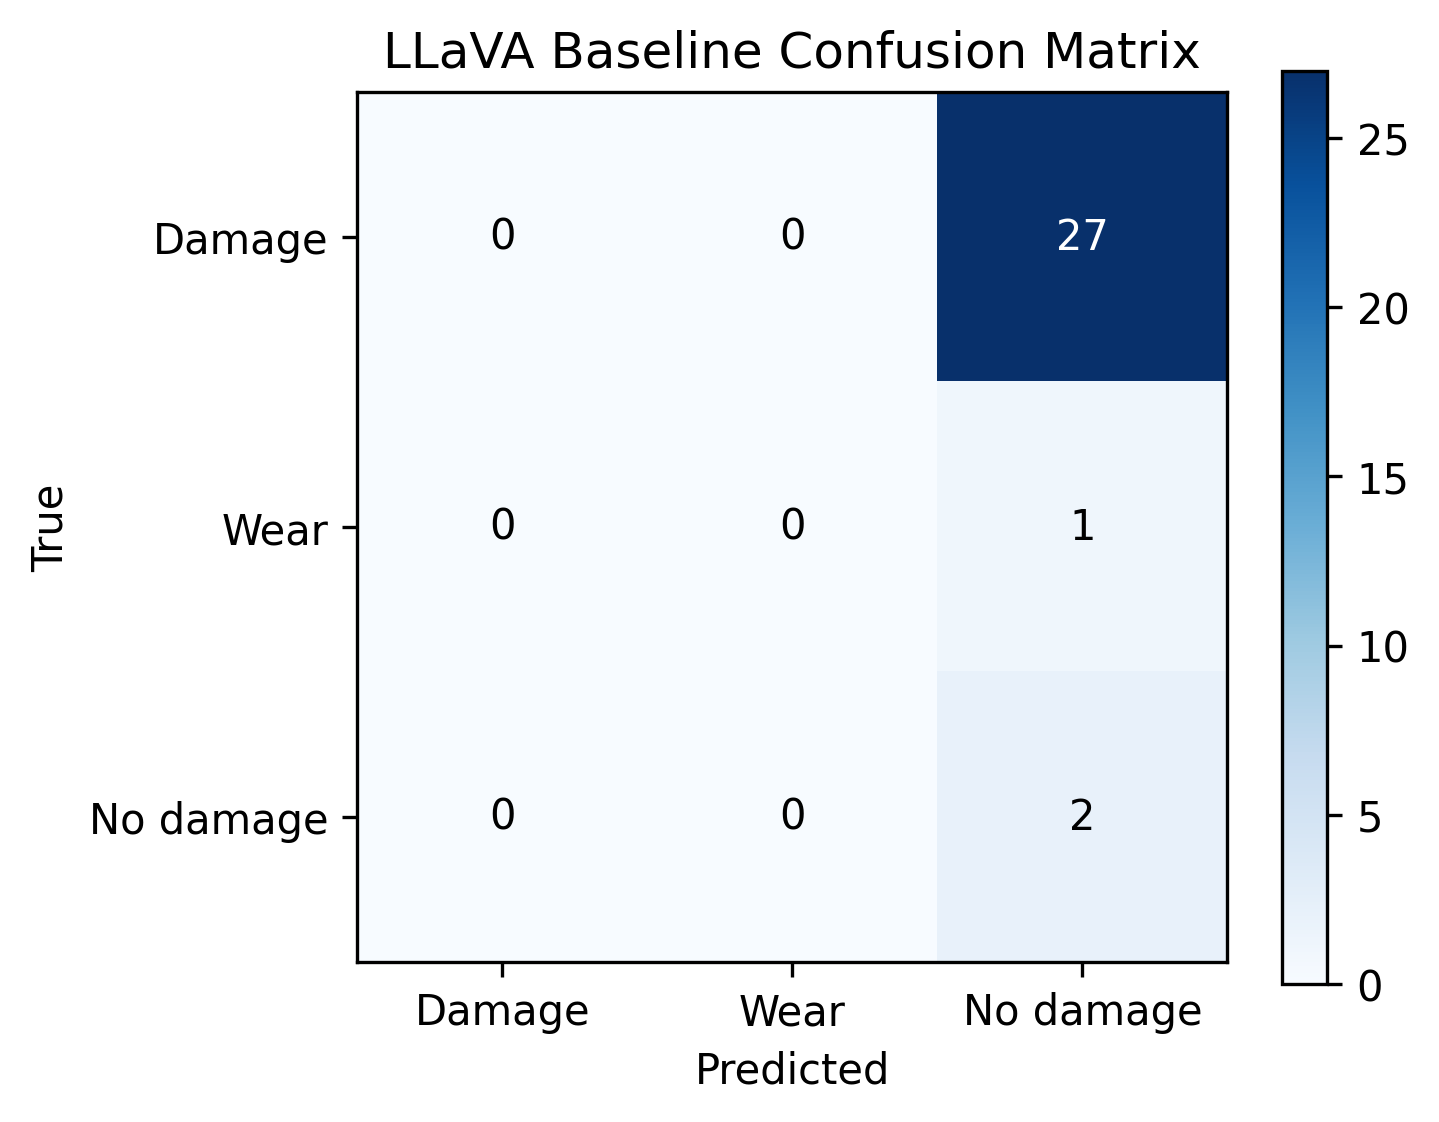
\includegraphics[width=\linewidth]{sections/2-thesis/llava_confusion_matrix.png}
\caption{LLaVA Baseline}
\label{fig:llava_baseline_cm}
\end{subfigure}

\vspace{0.5cm}

\begin{subfigure}{0.9\columnwidth}
\centering
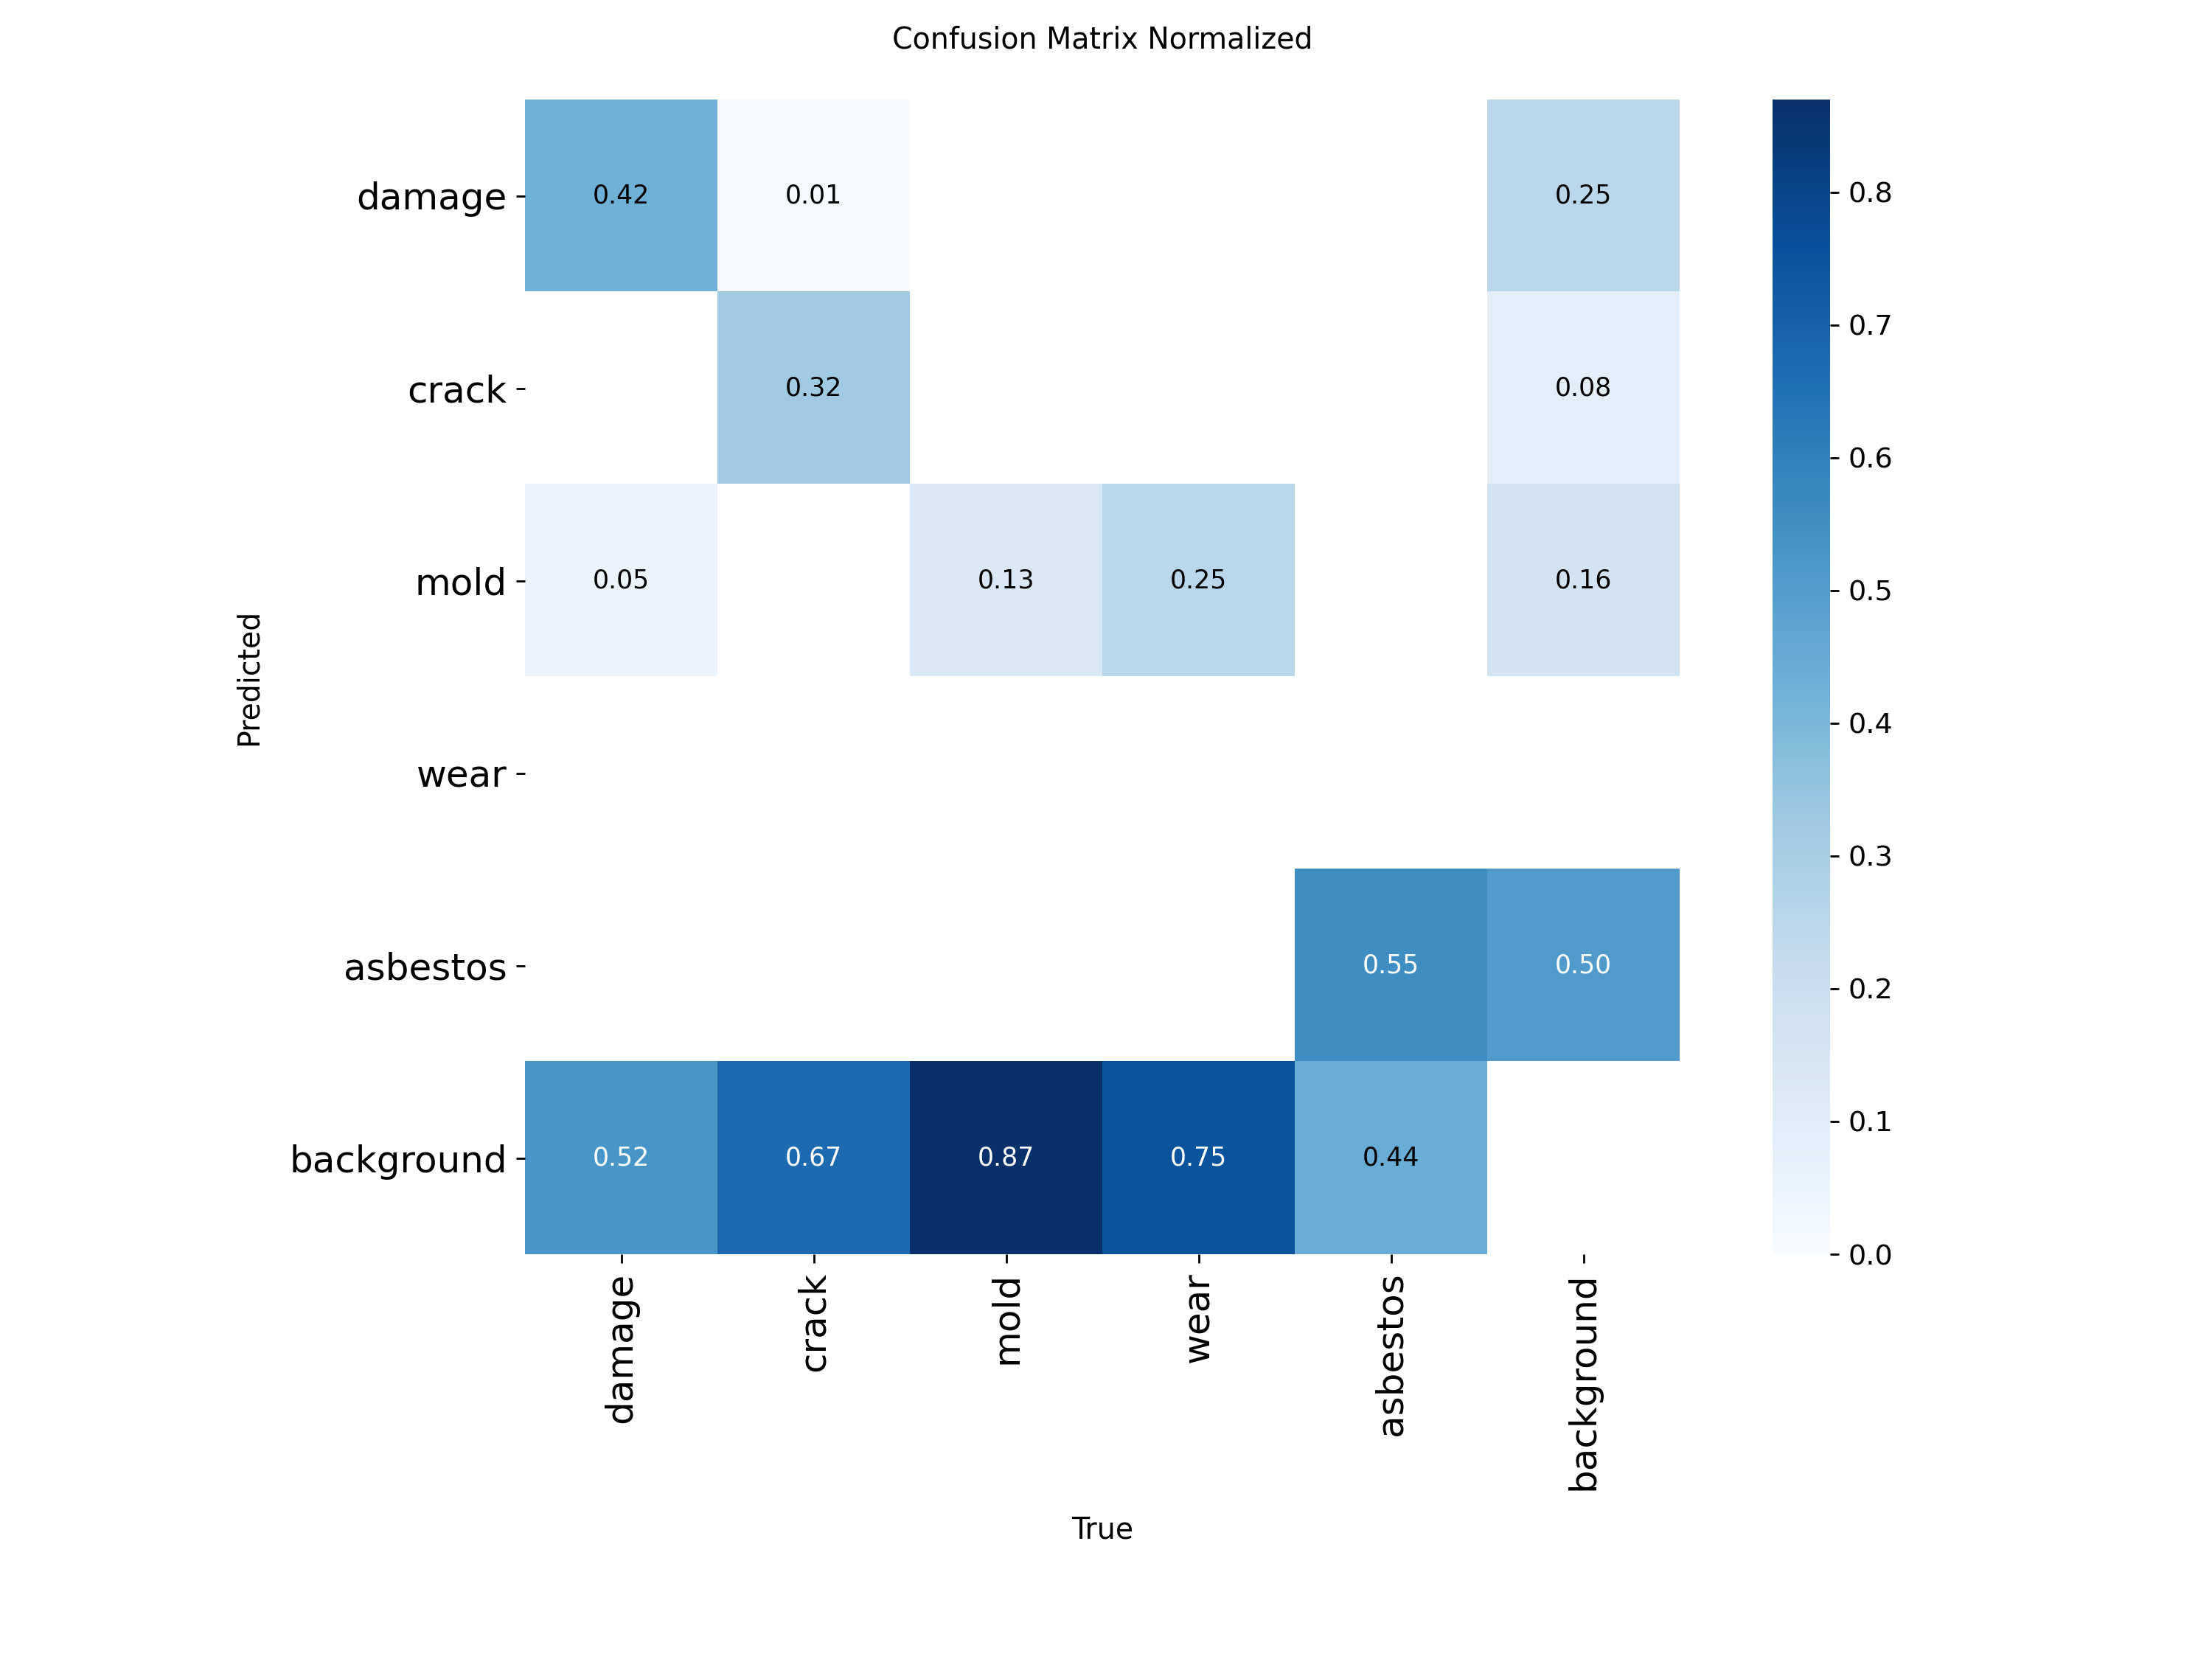
\includegraphics[width=\linewidth]{sections/2-thesis/yolo_baseline_confusion_matrix_normalized.png}

\caption{YOLOv8 Baseline}
\label{fig:yolo_baseline_cm}
\end{subfigure}

\caption{Confusion matrices of the baseline models.}
\label{fig:baseline_heatmaps}

\end{figure}

%                               

Table~\ref{tab:category_performance} summarizes the quantitative performance of the final YOLOv8 model, the LLaVA zero shot baseline, and the rule guided LLaVA configuration.

The results demonstrate clear performance differences between supervised object detection and multi modal zero shot reasoning. The YOLOv8 model achieved an overall F1 score of 0.138, while the LLaVA zero shot baseline achieved an overall F1 score of 0.265. Prompt optimization further improved LLaVA performance, resulting in an overall F1 score of 0.293. These results indicate that prompt engineering improved the performance of LLaVA, although both approaches have different strengths due to their fundamentally different prediction mechanisms.


\begin{table}[H]
\centering
\scriptsize
\renewcommand{\arraystretch}{1.15}
\caption{Performance per category for the evaluated models on the property level dataset.}
\label{tab:category_performance}
\begin{tabular}{p{1.8cm}p{1.4cm}p{1.4cm}p{1.4cm}}
\toprule
Category & Precision & Recall & F1 score \\
\midrule

\multicolumn{4}{l}{\textbf{YOLOv8}}\\
\midrule
Overall & 0.114 & 0.174 & 0.138 \\
Damage & 0.239 & 0.355 & 0.286 \\
Crack & 0.000 & 0.000 & 0.000 \\
Mold & 0.000 & 0.000 & 0.000 \\
Wear & 0.000 & 0.000 & 0.000 \\
Asbestos & 0.000 & 0.000 & 0.000 \\
No damage & 0.447 & 0.689 & 0.543 \\

\midrule
\multicolumn{4}{l}{\textbf{LLaVA Zero Shot}}\\
\midrule
Overall & 0.553 & 0.263 & 0.265 \\
Damage & 1.000 & 0.194 & 0.324 \\
Crack & 1.000 & 0.059 & 0.111 \\
Mold & 0.333 & 0.167 & 0.222 \\
Wear & 0.455 & 0.161 & 0.238 \\
Asbestos & 0.000 & 0.000 & 0.000 \\
No damage & 0.532 & 1.000 & 0.695 \\

\midrule
\multicolumn{4}{l}{\textbf{LLaVA Rule Guided}}\\
\midrule
Overall & 0.454 & 0.245 & 0.293 \\
Damage & 1.000 & 0.161 & 0.278 \\
Crack & 0.067 & 0.059 & 0.062 \\
Mold & 0.333 & 0.167 & 0.222 \\
Wear & 0.440 & 0.355 & 0.393 \\
Asbestos & 0.41 & 0.41 & 0.41 \\
No damage & 0.885 & 0.730 & 0.800 \\

\bottomrule
\end{tabular}
\end{table}
%                                        

Prompt optimization improved LLaVA performance, increasing the F1 score from 0.125 to 0.155. However, the improvement remained limited and performance continued to lag behind the supervised detector. The final LLaVA 1.6 configuration achieved an overall F1 score of 0.147, suggesting that additional prompt refinement alone was insufficient to close the performance gap.

For the final YOLOv8 model, performance varied across inspection categories. The highest recall was achieved for the asbestos category (0.55), followed by no damage (0.50) and damage (0.42). Lower recall values were observed for mold (0.13) and wear (0.00), indicating that these categories remained more challenging to detect.

Overall, the results show that YOLOv8 benefited substantially from task specific supervision and bounding box annotations, whereas LLaVA struggled to reliably identify inspection categories using zero shot multi modal reasoning alone.

Across all evaluated configurations, YOLOv8 achieved higher precision, recall, and F1 score than LLaVA 1.6. Although prompt optimization improved the performance of LLaVA, the gap between both approaches remained substantial.

% add barchart YOLO vs llava

\subsubsection{SRQ2 Robustness under real world variability}

\textbf{SRQ2:} How robust are YOLOv8 and LLaVA when evaluated on a heterogeneous housing inspection dataset containing variation in image quality, lighting conditions, and viewing angles?

To evaluate robustness under realistic housing inspection conditions, the models were tested on eight independent DGW properties. The properties contain different inspection scenarios, including varying room layouts, viewing angles, lighting conditions, image quality, and levels of deterioration. Together, these properties provide a heterogeneous evaluation dataset that reflects practical housing inspections.

The complete ground truth distribution for each property before and after the lease period is presented in Appendix~\ref{appendix:property_ground_truth}. The appendix shows that the evaluation dataset contains properties that improved, remained unchanged, and deteriorated after the lease period. This variation ensures that the robustness evaluation is based on diverse inspection scenarios rather than on a single property.

The performance of both models across the individual properties is presented in Table~\ref{tab:property_performance}. The quantitative results are used to assess the consistency of each model under different inspection conditions.

%  still need to generate report performance for every house.
\begin{table}[ht]
\centering
\caption{Property level comparison between the ground truth and model predictions.}
\label{tab:propertycomparison}
\footnotesize
\begin{tabular}{lcccc}
\toprule
Property & Ground truth & YOLO & Zero Shot & Rule Guided \\
\midrule
001 & Worse & Worse & Worse & Worse \\
002 & Worse & Worse & Worse & Worse \\
003 & Worse & Worse & Improved & Worse \\
004 & Improved & Improved & Improved & Improved \\
005 & Stayed the same & Worse & Stayed the same & Stayed the same \\
006 & Stayed the same & Worse & Stayed the same & Stayed the same \\
007 & Stayed the same & Worse & Stayed the same & Stayed the same \\
008 & Improved & Improved & Improved & Improved \\
\midrule
Accuracy & -- & 75.0\% & 87.5\% & 100.0\% \\
\bottomrule
\end{tabular}
\end{table}
%\\\\\\\\\\\\\\\\\\\\\\\\\\\\\\\\\\\\
\subsubsection{SRQ3 Practical advantages and limitations}

\textbf{SRQ3:} Which practical differences between YOLOv8 and LLaVA 1.6 were observed during the experiments?

Besides quantitative performance, the experiments also provide insight into the practical characteristics of both approaches. Table~\ref{tab:practical_comparison} summarizes the main observations made during model development and evaluation.

\begin{table}[H]
\centering
\small
\caption{Practical comparison between YOLOv8 and LLaVA 1.6.}
\label{tab:practical_comparison}
\begin{tabular}{p{1.8cm}p{2cm}p{2cm}}
\toprule
Characteristic & YOLOv8 & LLaVA \\
\midrule
Training & Required & Not required \\
Zero shot & No & Yes \\
Localization & Bounding boxes & None \\
Output & Structured & Natural language \\
Prompting & No & Yes \\
Consistency & Higher & Lower \\
\bottomrule
\end{tabular}
\end{table}

The results show clear practical differences between both model paradigms. YOLOv8 requires task specific training before deployment but produces structured object detections with precise localization of inspection relevant categories\cite{redmon_you_2016,jocher_ultralytics_2023}. In contrast, LLaVA 1.6 can be applied without additional training through zero shot prompting, producing natural language descriptions that require post processing before evaluation\cite{liu_visual_2023}.

Across all experiments, YOLOv8 produced more consistent predictions and achieved higher quantitative performance than LLaVA 1.6. Although LLaVA offers greater flexibility through zero shot inference, its predictions depended on prompt design and remained less consistent than those of the supervised detector. These observations provide practical evidence regarding the suitability of both approaches for housing inspection workflows.

\section{Summary of Results}

The experimental results provide evidence for all three sub research questions. For SRQ1, YOLOv8 consistently achieved higher performance than LLaVA 1.6 across all evaluated configurations and inspection categories. For SRQ2, both models were evaluated on a heterogeneous set of housing inspection properties representing different inspection scenarios, enabling the assessment of robustness under realistic conditions. For SRQ3, the experiments demonstrated clear practical differences between both approaches, with YOLOv8 providing structured object localization after task specific training and LLaVA offering zero shot capabilities through prompt based reasoning.

Together, these findings provide the experimental evidence used to answer the main research question. Their implications are discussed in the following chapter.

